\subsection{Block Flux Memory}\label{sec:memory-structure}

In the current implementation of \gls{hms}, only state variables are stored in memory, as all other variables are computed from the previous state. 
Other variables, like fluxes, are temporarily stored in solver thread buffers.
Thus, to enable reuse of fluxes, an additional memory structure is needed.
A two stage approach was chosen for this task:
Firstly, the implementation of a structure \texttt{BlockFluxes}, which stores fluxes and expiry time for each block;
secondly, the creation of a class \texttt{BlockFluxMemory}, which manages \texttt{BlockFluxes} objects and implements the concept of a \acrlong{bfm}. 
It stores a \texttt{std::vector} of \texttt{BlockFluxes} and various member variables which help to index the blocks. 
\texttt{BlockFluxMemory} provides access functions for \texttt{BlockFluxes} objects and all relevant member variables, as well as a function to determine whether a neighbor block requires a full computation to enable neighbor propagation.

Since \gls{hms} supports both first-order and \gls{tvd} reconstruction, the \acrlong{bfm} needs to adapt to either option's partitioning scheme.

\begin{figure}[!b]
  \centering
  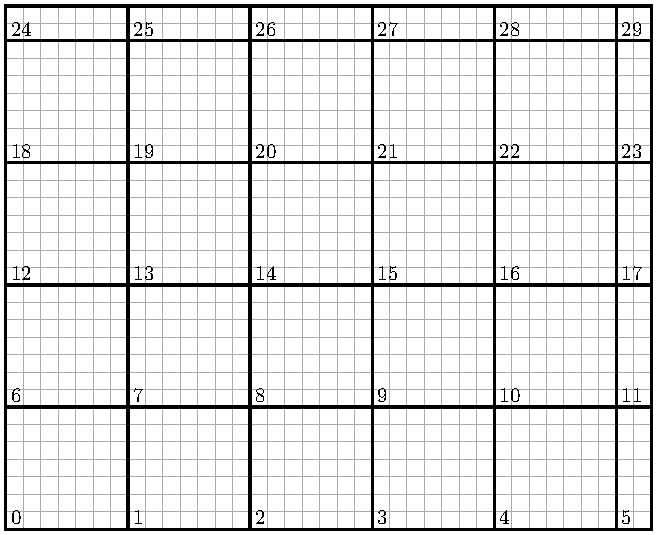
\includegraphics[width=0.7\textwidth]{../typst/bfm-index/bfm-index-fo.pdf}
  \caption[\Acrlong{bfm}: Block map for first-order scheme]{
    \Acrlong{bfm}: Block map for the use with a first-order scheme.
    Cell boundaries are drawn as gray lines, whereas the block boundaries are depicted in black.
    The block index is shown in each block's bottom-left corner.
    Block size: $7 \times 7$ cells, mesh size: $37 \times 30$ cells.
  }
  \label{fig:bfm-index-fo}
\end{figure}

% Block partitioning for the first-order scheme is rather simple, as there are no boundary blocks. 
When using first-order reconstruction, the mesh is partitioned into blocks of fixed, user-specifiable sizes and smaller remainder blocks, as shown in \autoref{fig:bfm-index-fo}.
Starting from the bottom-left corner, the domain is filled with full blocks. 
Block size is not required to adapt to mesh size; thus, possible remaining cells are covered with smaller remainder blocks.

In contrast, block-wise traversal for the \gls{tvd} scheme requires a layer of blocks wrapping the mesh's boundary, having a fixed width of two cells.
This is due to the nature of second-order schemes, which take derivates of multiple cells' values around an edge into account to compute the fluxes over that edge.
Narrow blocks enable correct usage of the \gls{tvd} scheme at the domains boundaries.
A more complex partitioning scheme than for the first-order scheme results of this, as shown in \autoref{fig:bfm-index-tvd}.

\begin{figure}[!b]
  \centering
  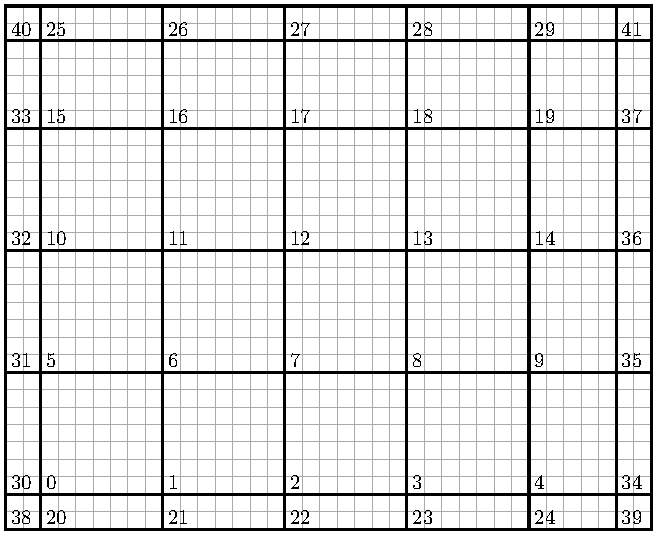
\includegraphics[width=0.7\textwidth]{../typst/bfm-index/bfm-index-tvd.pdf}
  \caption[\Acrlong{bfm}: Block map for \acrshort{tvd} scheme]{
    \Acrlong{bfm}: Block map for the use with a \acrshort{tvd} scheme.
    Cell boundaries are drawn as gray lines, whereas the block boundaries are depicted in black.
    The block index is shown in each block's bottom-left corner.
    Block size: $7 \times 7$ cells, mesh size: $37 \times 30$ cells, boundary layer width: $2$ cells.
  }
  \label{fig:bfm-index-tvd}
\end{figure}

Currently, \gls{hms} identifies blocks by the coordinate of the cell in their bottom-left corner.
Thus, the \acrlong{bfm} needs to introduce an indexing mechanism according to both partitioning schemes for accessing \texttt{BlockFluxes} based block coordinates.
% , which is done by starting with inner blocks, including their remainders, followed by bottom, top, left and right boundary blocks, and finally corner blocks.
% To enable performant indexing, \gls{bfm} stores start index and number of blocks for each \texttt{BlockLocation}, which are assigned during initialization of a \gls{bfm} object and are accessed using the \texttt{blockIndex(\dots)} member function.
An additional \gls{2D} vector stores all block index numbers in a two-dimensional representation for efficiently retrieving adjacent blocks. 
% The location for each block in this 2D vector is stored in \texttt{BlockFluxes}.

The \gls{bfm} is instantiated at the start of each run of a \gls{hms} before the time loop starts.
Upon initialization, member variables for block indexing are populated, a \texttt{BlockFluxes} object for each block is constructed, and stored in a vector, at the position corresponding to its block index.
% Existing functions for computing blocks in \gls{hms} were adapted to utilize \gls{bfm} access functions for storing and reusing precomputed fluxes, as explained in \autoref{sec:time-step-scheme}.
% After finishing the time loop, a logger is used to output a summary for all blocks, which is used to generate a statistic as shown later in {fig:heatmap-dambreak}.